\chapter{高中数学若干问题}
这一章主要记录本人在读高中的时候处理一些典型数学问题的方法,用以提高大家的数学计算能力.同时也为了表明一个物理老师的是如何处理数学问题的,相信同学们在仔细钻研后肯定有所收获.
\section{对称点问题和点到直线的距离}
记直线L的某一由$(x_2,y_2)$指向$(x_1,y_1)$的法向量$\vec{n}$,则$\vec{n}$与$(x_1-x_2,y_1-y_2)$平行.$(x_0,y_0)$为L上任意一点,则$(x_1-x_0,y_1-y_0)\cdot \vec{n}$为$(x_1,y_1)$到L的距离.如图\ref{fig:duichengdian}所示
\begin{figure}[H]
  \centering
  \begin{tikzpicture}
    \draw[->,>=stealth](-3,0)--(3,0) node [anchor=north]{\small x};
    \draw[->,>=stealth](0,-3)--(0,3) node [anchor=west]{\small y};
    \draw (-1,-2)--(3,2);
    \filldraw(0.5,-0.5) circle [radius=1pt] node [anchor=south east] {\tiny $(x_0,y_0)$};
    \filldraw(0.5,1) circle [radius=1pt] node [anchor=south east]{\tiny $(x_1,y_1)$};
    \filldraw(2,-0.5) circle [radius=1pt] node [anchor=north west]{\tiny $(x_2,y_2)$};
    \draw [->,>=stealth](0.5,-0.5)--(0.5,1);
    \draw [->,>=stealth](2,-0.5)--(0.5,1);
  \end{tikzpicture}
  \caption{对称点问题}
  \label{fig:duichengdian}
\end{figure}

\begin{gather}
  \intertext{下面再来研究$(x_1,y_1)$与$(x_2,y_2)$关于L对称.则$(x_1-x_2,y_1-y_2)$的模是$(x_1,y_1)$到L距离的$2$倍,则}
  (x_1-x_2,y_1-y_2)=2(x_1-x_0,y_1-y_0)\cdot \vec{n}\vec{n}
  \intertext{看上式的右式,如将$\vec{n'}=-\vec{n}$作替换,则有}
  (x_1-x_2,y_1-y_2)=2(x_1-x_0,y_1-y_0)\cdot \vec{n}\vec{n}=2(x_1-x_0,y_1-y_0)\cdot\vec{n'}\vec{n'}
  \intertext{上式表明无论是$\vec{n}$还是$\vec{n'}$,不需要考虑其方向由$(x_1,y1)$指向$(x_2,y_2)$还是由$(x_2,y_2)$指向$(x_1,y_1)$则等式永远成立.于是可以取L的一个法向量为}
  \vec{n}=\frac{(A,B)}{\sqrt{A^2+B^2}}
  \intertext{则有}
  (x_1-x_2,y_1-y_2)=2(x_1-x_0,y_1-y_0)\cdot\frac{(A,B)}{\sqrt{A^2+B^2}}\frac{(A,B)}{\sqrt{A^2+B^2}}\\
  (x_1-x_2,y_1-y_2)=2\frac{Ax_1+By_1+C}{A^2+B^2}(A,B)
  \intertext{解得}
  x_2=x_1-\frac{2A}{A^2+B^2}(Ax_1+Bx_1+C)\\
  y_2=y_1-\frac{2B}{A^2+B^2}(Ax_1+Bx_1+C)
  \intertext{若$(x_1,y_1)$为已知点,则由此公式可以方便的求出对称点.同时可以求出点到直线的距离$d$为}
d=|(x_1-x_0,y_1-y_0)\cdot\vec{n}|
\intertext{即}
d=\frac{|Ax_1+By_1+C|}{\sqrt{A^2+B^2}}
\intertext{注意:上式中由于$(x_0,y_0)$在L上,则$Ax_0+B_0+C=0$于是有$C=-Ax_0-By_0$.}\notag
\end{gather}
\section{立体几何的二面角的求解}
\subsection{三角公式法}
如图所示,记平面$\Sigma$和平面$\Sigma$二面角为$\gamma$则
\begin{figure}[H]
  \centering
  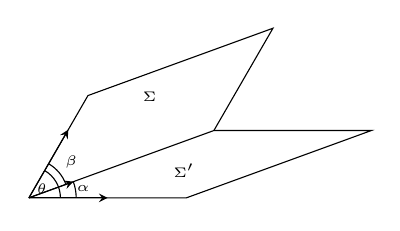
\begin{tikzpicture}
    \draw(0,0)--(0:2)--++(20:2.5)--++(180:2);
    \draw(0,0)--(20:2.5);
    \draw(0,0)--(60:1.5)--++(20:2.5)--++(240:1.5);
    \draw[->,>=stealth](0,0)--(0:1);
    \draw[->,>=stealth](0,0)--(20:0.6);
    \draw[->,>=stealth](0,0)--(60:1);
    \draw (0:0.4) arc (0:60:0.4);
    \draw (0:0.6) arc (0:20:0.6);
    \draw (20:0.5) arc (20:60:0.5);
    \draw (35:0.2) node {\tiny $\theta$};
    \draw (10:0.7) node {\tiny $\alpha$};
    \draw (40:0.7) node {\tiny $\beta$};
    \draw (10:2) node {\tiny $\Sigma'$};
    \draw (40:2) node {\tiny $\Sigma$};
  \end{tikzpicture}
  \caption{三角公式法}
  \label{fig:ermianjiao1}
\end{figure}
\begin{gather}
  (\vec{n_2}-\vec{n_2}\cdot\vec{n}\vec{n})\cdot(\vec{n_1}-\vec{n_1}\cdot\vec{n}\vec{n})=\sin\alpha\sin\beta\cos\gamma\\
  \vec{n_2}\cdot\vec{n_1}-\vec{n_1}\cdot\vec{n}\vec{n_2}\cdot\vec{n}-\vec{n_2}\cdot\vec{n}\vec{n_1}\cdot\vec{n}+\vec{n_1}\cdot\vec{n}\vec{n_2}\cdot\vec{n}=\sin\alpha\sin\beta\cos\gamma\\
  \cos\theta-\cos\alpha\cos\beta=\sin\alpha\sin\beta\cdot\cos\gamma\\
  \cos\gamma=\frac{\cos\theta-\cos\alpha\cos\beta}{\sin\alpha\sin\beta}
  \intertext{知道角$\alpha,\beta,\theta$可直接算出$\gamma$的余弦值.}\notag
\end{gather}
\subsection{采用内积的坐标算法}
如图\ref{fig:ermianjiao2}所示,遇到立体几何问题要毫不犹豫的写出以下 o,A,B,C几个点的坐标,其中$OB$为平面$\Sigma$和平面$\Sigma'$的交线.作$CC'\bot OB$于$C'$,$A'A\bot OB$于$A'$.
\begin{gather}
  \intertext{类比上一节的计算可得}
  \overset{\longrightarrow}{C'C}=\overset{\longrightarrow}{OC}-\frac{\overset{\longrightarrow}{OC}\cdot \overset{\longrightarrow}{OB}}{|\overset{\longrightarrow}{OB}|^2}\overset{\longrightarrow}{OB}
  \intertext{同理}
  \overset{\longrightarrow}{A'A}=\overset{\longrightarrow}{OA}-\frac{\overset{\longrightarrow}{OA}\cdot \overset{\longrightarrow}{OB}}{|\overset{\longrightarrow}{OB}|^2}\overset{\longrightarrow}{OB}
  \intertext{于是$\Sigma$和$\Sigma'$的夹角$\gamma$为}
  \cos\gamma=\frac{\overset{\longrightarrow}{C'C}\cdot\overset{\longrightarrow}{A'A}}{|\overset{\longrightarrow}{C'C}|\cdot|\overset{\longrightarrow}{A'A}|}
  \intertext{注意:所有这些都要用坐标运算,不需要多做考虑,对于应对高考的数学解析几何是一个相当大的优势.}\notag
\end{gather}
\begin{figure}[H]
  \centering
  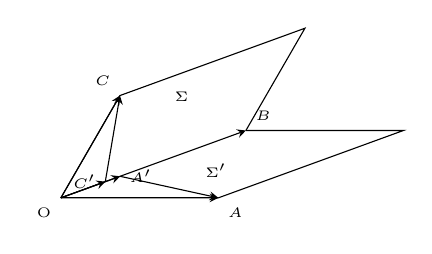
\begin{tikzpicture}
    \draw(0,0)--(0:2)--++(20:2.5)--++(180:2);
    \draw[->,>=stealth](0,0)--(20:2.5) node [anchor=south west]{\tiny $B$};
    \draw(0,0)--(60:1.5)--++(20:2.5)--++(240:1.5);
    \draw[->,>=stealth](0,0)--(0:2) node [anchor=north west]{\tiny $A$};
    \draw[->,>=stealth](0,0)--(20:0.6) node [anchor=east]{\tiny $C'$};
    \draw[->,>=stealth](0,0)--(60:1.5) node [anchor=south east]{\tiny $C$};
    \draw(0,0) node [anchor=north east]{\tiny O};
    \draw[->,>=stealth](20:0.6)--(60:1.5);
    \draw[->,>=stealth](0,0)--(20:0.8) node [anchor=west]{\tiny $A'$};
    \draw[->,>=stealth](20:0.8)--(0:2);
    \draw (10:2) node {\tiny $\Sigma'$};
    \draw (40:2) node {\tiny $\Sigma$};
  \end{tikzpicture}
  \caption{坐标算法}
  \label{fig:ermianjiao2}
\end{figure}
\subsection{采用外积的坐标算法}
外积的定义为:
\begin{equation}
  \vec{a}\times\vec{b}=ab\sin\theta \vec{n}
\end{equation}
\begin{figure}[H]
  \centering
  \begin{tikzpicture}
  \draw[->,>=stealth](0,0)--(0:2) node [anchor=west]{\tiny $\vec{a}$};
  \draw[->,>=stealth](0,0)--(20:2) node [anchor=south]{\tiny $\vec{b}$};
  \draw[->,>=stealth](0,0)--(90:1) node [anchor=east]{\tiny $\vec{n}$};
  \draw[->,>=stealth](0:1) arc (0:20:1);
  \draw[pattern=north west lines](0,0)--++(0:2)--++(20:2)--++(180:2)--++(200:2);
  \draw (8:1.3) node {\tiny $\theta$};
  \end{tikzpicture}
  \caption{外积的方向}
  \label{fig:waiji}
\end{figure}
其中$\vec{n}$垂直于$\vec{a}$和$\vec{b}$所在平面,外积是一个矢量,它的大小为图\ref{fig:waiji}所示的阴影的面积,方向就是$\vec{n}$的方向.

\subsection{矢量外积的坐标式}
\begin{gather}
\intertext{记$\vec{a}=(a_1,a_2,a_3)$,$\vec{b}=(b_1,b_2,b_3)$则}
\vec{a}\times\vec{b}=
\begin{vmatrix}
  \vec{i}&\vec{j}&\vec{k}\\
  a_1&a_2&a_3\\
  b_1&b_2&b_3
\end{vmatrix}
=
\begin{vmatrix}
  a_2&a_3\\
  b_2&b_3
\end{vmatrix}\vec{i}
-
\begin{vmatrix}
  a_1&a_3\\
  b_1&b_3
\end{vmatrix}\vec{j}
+
\begin{vmatrix}
  a_1&a_2\\
  b_1&b_2
\end{vmatrix}\vec{k}
\intertext{例:外积的计算,如果$\vec{a}=(1,1,2),\vec{b}=(1,0,3)$则}
\vec{a}\times\vec{b}=
\begin{vmatrix}
  \vec{i}&\vec{j}&\vec{k}\\
  1&1&2\\
  1&0&3
\end{vmatrix}
=
\begin{vmatrix}
  1&2\\
  0&3
\end{vmatrix}\vec{i}
-
\begin{vmatrix}
  1&2\\
  1&3
\end{vmatrix}\vec{j}
+
\begin{vmatrix}
  1&1\\
  1&0
\end{vmatrix}\vec{k}\\
\vec{a}\times\vec{b}=3\vec{i}-\vec{j}-\vec{k}=(3,-1,-1)
\end{gather}

如图\ref{fig:waiji2}所示
\begin{figure}[H]
  \centering
  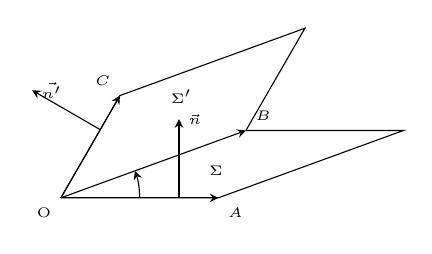
\begin{tikzpicture}
    \draw(0,0)--(0:2)--++(20:2.5)--++(180:2);
    \draw[->,>=stealth](0,0)--(20:2.5) node [anchor=south west]{\tiny $B$};
    \draw(0,0)--(60:1.5)--++(20:2.5)--++(240:1.5);
    \draw[->,>=stealth](0,0)--(0:2) node [anchor=north west]{\tiny $A$};
    \draw[->,>=stealth](0,0)--(60:1.5) node [anchor=south east]{\tiny $C$};
    \draw(0,0) node [anchor=north east]{\tiny O};
    \draw (10:2) node {\tiny $\Sigma$};
    \draw (40:2) node {\tiny $\Sigma'$};
    \draw [->,>=stealth] (0:1) arc (0:20:1);
    \draw [->,>=stealth] (0:1.5)--++(90:1) node [anchor=west]{\tiny $\vec{n}$};
    \draw [->,>=stealth] (60:1)--++(150:1) node [anchor=west]{\tiny $\vec{n'}$};
  \end{tikzpicture}
  \caption{外积计算二面角}
  \label{fig:waiji2}
\end{figure}

\begin{gather}
  \intertext{$\overset{\longrightarrow}{OA}$和$\overset{\longrightarrow}{OB}$,$\overset{\longrightarrow}{OC}$均可以用坐标方便的表示出来,无需考虑具体的几何关系,则}
  \vec{n}=\overset{\longrightarrow}{OA}\times\overset{\longrightarrow}{OB}\\
  \vec{n}=\overset{\longrightarrow}{OC}\times\overset{\longrightarrow}{OB}
  \intertext{则$\Sigma'$和$\Sigma$的夹角$\gamma$可以由它们的法向量$\vec{n}$和$\vec{n'}$示得,如下}
  \cos\gamma=\frac{\vec{n'}\cdot\vec{n}}{|\vec{n'}|\cdot|\vec{n}|}
  \intertext{注意:在所介绍的这三种方法中,外积法高中数学没有介绍,但是此法最简单,练熟后大题采用上式,则不用寻找具体的几何关系,可以直接写出答案.}\notag
\end{gather}
\section{三角函数变换公式}
关于三角函数问题要学会和、差、倍、半、万能公式的推理论证,否则此类问题将会消耗更多的时间.下面我详证这些关系.
首先由余弦定理导出差角公式,关于余弦公式前面在力的合成分解中已经详细论证了,这里不再赘述.如图\ref{fig:chajiao}所示
\begin{figure}[H]
  \centering
  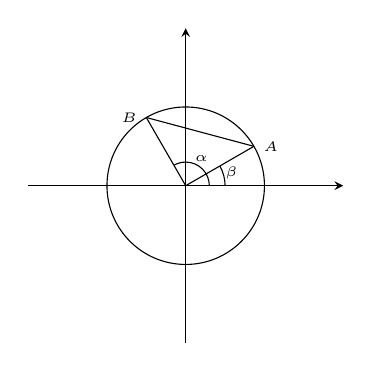
\begin{tikzpicture}
    \draw[->,>=stealth] (-2,0)--(2,0); 
    \draw[->,>=stealth] (0,-2)--(0,2); 
    \draw (0,0) circle [radius=1];
    \draw (0,0)--(30:1) node [anchor=west]{\tiny $A$};
    \draw (0,0)--(120:1) node [anchor=east]{\tiny $B$};
    \draw(30:1)--(120:1);
    \draw (0:0.5) arc (0:30:0.5);
    \draw (0:0.3) arc (0:120:0.3);
    \draw (15:0.6) node {\tiny $\beta$};
    \draw (60:0.4) node {\tiny $\alpha$};
  \end{tikzpicture}
  \caption{差角公式}
  \label{fig:chajiao}
\end{figure}
\begin{gather}
  \intertext{由图\ref{fig:chajiao}可知$A(\cos\beta,\sin\beta)$,$B(\cos\alpha,\sin\alpha)$,再由余弦定理可得}
  (\cos\alpha-\cos\beta)^2+(\sin\alpha-\sin\beta)^2=1+1-2\cos(\alpha-\beta)\notag\\
  \cos(\alpha-\beta)=\cos\alpha\cos\beta+\sin\alpha\sin\beta
  \label{eq:chajiao0}
  \intertext{上式中取$\beta$替换为$-\beta$得}
  \cos(\alpha+\beta)=\cos\alpha\cos\beta-\sin\alpha\sin\beta
  \label{eq:chajiao1}
  \intertext{对式\eqref{eq:chajiao1}将$\alpha$视为变量$\beta$视为常量,对$\alpha$求导则}
  -\sin(\alpha+\beta)=-\sin\alpha\cos\beta-\cos\alpha\sin\beta\notag\\
  \sin(\alpha+\beta)=\sin\alpha\cos\beta\cos\alpha\sin\beta
  \intertext{同理对式\eqref{eq:chajiao0}将$\alpha$视为变量$\beta$视为常量,对$\alpha$求导得}
  -\sin(\alpha-\beta)=-\sin\alpha\cos\beta+\cos\alpha\sin\beta\notag\\
  \sin(\alpha-\beta)=\sin\alpha\cos\beta-\cos\alpha\sin\beta
  \intertext{综上所述,得{\bf 和角公式}为}
  \left\{
    \begin{gathered}
      \sin(\alpha+\beta)=\sin\alpha\cos\beta+\cos\alpha\sin\beta\\
      \cos(\alpha+\beta)=\cos\alpha\cos\beta-\sin\alpha\sin\beta
    \end{gathered}
  \right.
  \label{eq:hejiao}
  \intertext{{\bf 差角公式}为}
  \left\{
    \begin{gathered}
      \sin(\alpha-\beta)=\sin\alpha\cos\beta-\cos\alpha\sin\beta\\
      \cos(\alpha-\beta)=\cos\alpha\cos\beta+\sin\alpha\sin\beta
    \end{gathered}
  \right.
  \label{eq:chajiao}
  \intertext{取$\alpha=\beta$代入和角公式\eqref{eq:hejiao}得{\bf 倍角公式}}
  \left\{
    \begin{gathered}
      \sin2\alpha=2\sin\alpha\cos\alpha\\
      \cos2\alpha=\cos^2\alpha-\sin^2\alpha
    \end{gathered}
  \right.
  \label{eq:beijiao}
  \intertext{考虑到$\sin^2\alpha+\cos^2\alpha=1$得}
  \cos2\alpha=1-2\sin^2\alpha\notag\\
  \label{eq:beijiao0}
  \sin\alpha=\pm\sqrt{\frac{1-\cos2\alpha}{2}}
  \intertext{上式中$\pm$取决于$\alpha$的象限,取$\frac{\alpha}{2}$代换$\alpha$得}
  \sin\frac{\alpha}{2}=\pm\sqrt{\frac{1-\cos\alpha}{2}}
  \intertext{同理由\eqref{eq:beijiao}可得}
  \cos2\alpha=2\cos^2\alpha-1\notag\\
  \cos\alpha=\pm\sqrt{\frac{1+\cos2\alpha}{2}}
  \intertext{同理令$\frac{\alpha}{2}$取代$\alpha$得}
  \cos\frac{\alpha}{2}=\pm\sqrt{\frac{1+\cos\alpha}{2}}
  \intertext{写到一块得{\bf 半角公式}}
  \left\{
    \begin{gathered}
      \sin\frac{\alpha}{2}=\pm\sqrt{\frac{1-\cos\alpha}{2}}\\
      \cos\frac{\alpha}{2}=\pm\sqrt{\frac{1+\cos\alpha}{2}}
    \end{gathered}
    \right.
    \intertext{下面论证万能公式}
    \tan(\alpha+\beta)=\frac{\sin(\alpha+\beta)}{\cos(\alpha+\beta)}=\frac{\sin\alpha\cos\beta+\cos\alpha\sin\beta}{\cos\alpha\cos\beta-\sin\alpha\sin\beta}
    \intertext{上式分子分母同时除以$\cos\alpha\cos\beta$得{\bf 万能公式第一式}}
    \tan(\alpha+\beta)=\frac{\tan\alpha+\tan\beta}{1-\tan\alpha\tan\beta}
    \label{eq:wanneng0}
    \intertext{上式\eqref{eq:wanneng0}中令$\beta$替换为$-\beta$则}
    \tan(\alpha-\beta)=\frac{\tan\alpha-\tan\beta}{1+\tan\alpha\tan\beta}
    \label{eq:wanneng1}
    \intertext{式\eqref{eq:wanneng0}中令$\alpha=\beta$则}
    \tan2\alpha=\frac{2\tan\alpha}{1-\tan^2\alpha}
    \intertext{上式中令$\alpha$代换为$\frac{\alpha}{2}$}
    \tan\alpha=\frac{2\tan\frac{\alpha}{2}}{1-\tan^2\frac{\alpha}{2}}
    \intertext{同时}
    \sin\alpha=2\sin\frac{\alpha}{2}\cos\frac{\alpha}{2}=\frac{2\sin\frac{\alpha}{2}\cos\frac{\alpha}{2}}{\sin^2\frac{\alpha}{2}+\cos^2\frac{\alpha}{2}}=\frac{2\tan\frac{\alpha}{2}}{1+\tan^2\frac{\alpha}{2}}\\
    \cos\alpha=\frac{\sin\alpha}{\tan\alpha}=\frac{1-\tan^2\frac{\alpha}{2}}{1+\tan^2\frac{\alpha}{2}}
    \intertext{通过上面的论证,我们把$\tan\alpha,\sin\alpha,\cos\alpha$都表达成了$\tan\frac{\alpha}{2}$的函数,所以原则上所有的三角函数都可以表达成$\tan\frac{\alpha}{2}$的函数,基于这个原因我们把下面这组式称为{\bf 万能公式}}
    \begin{gathered}
      \tan\alpha=\frac{2\tan\frac{\alpha}{2}}{1-\tan^2\frac{\alpha}{2}}\\
      \sin\alpha=\frac{2\tan\frac{\alpha}{2}}{1+\tan^2\frac{\alpha}{2}}\\
      \cos\alpha=\frac{1-\tan^2\frac{\alpha}{2}}{1+\tan^2\frac{\alpha}{2}}
    \end{gathered}
    \intertext{这几个公式在不定积分中有重要的应用,所以也是必须掌握的.为了清析起见,这里分组列出这几个重要的公式.}\notag
  \end{gather}
  \begin{gather}
    \intertext{{\bf 和角公式:}}
  \left\{
    \begin{gathered}
      \sin(\alpha+\beta)=\sin\alpha\cos\beta+\cos\alpha\sin\beta\\
      \cos(\alpha+\beta)=\cos\alpha\cos\beta-\sin\alpha\sin\beta\\
      \tan(\alpha+\beta)=\frac{\tan\alpha+\tan\beta}{1-\tan\alpha\tan\beta}
    \end{gathered}
  \right.\\
  \intertext{{\bf 差角公式:}}
  \left\{
    \begin{gathered}
      \sin(\alpha-\beta)=\sin\alpha\cos\beta-\cos\alpha\sin\beta\\
      \cos(\alpha-\beta)=\cos\alpha\cos\beta+\sin\alpha\sin\beta\\
      \tan(\alpha-\beta)=\frac{\tan\alpha-\tan\beta}{1+\tan\alpha\tan\beta}
    \end{gathered}
  \right.\\
  \intertext{{\bf 倍角公式:}}
  \left\{
    \begin{gathered}
      \sin2\alpha=2\sin\alpha\cos\alpha\\
      \cos2\alpha=\cos^2\alpha-\sin^2\alpha\\
      \tan2\alpha=\frac{2\tan\alpha}{1-\tan^2\alpha}
    \end{gathered}
  \right.
  \intertext{{\bf 半角公式:}}
  \left\{
    \begin{gathered}
      \sin\frac{\alpha}{2}=\pm\sqrt{\frac{1-\cos\alpha}{2}}\\
      \cos\frac{\alpha}{2}=\pm\sqrt{\frac{1+\cos\alpha}{2}}\\
      \tan\frac{\alpha}{2}=\pm\sqrt{\frac{1-\cos\alpha}{1+\cos\alpha}}
    \end{gathered}
  \right.\\
  \intertext{{\bf 万能公式:}}
  \begin{gathered}
    \tan\alpha=\frac{2\tan\frac{\alpha}{2}}{1-\tan^2\frac{\alpha}{2}}\\
    \sin\alpha=\frac{2\tan\frac{\alpha}{2}}{1+\tan^2\frac{\alpha}{2}}\\
    \cos\alpha=\frac{1-\tan^2\frac{\alpha}{2}}{1+\tan^2\frac{\alpha}{2}}
  \end{gathered}
\end{gather}
\section{数列问题}
\subsection{三个基本数列}
\begin{gather}
  \intertext{采用倒序相加可得自然数前n项和}
  \sum_{i=1}^n i=1+2+3+\cdots +n=\frac{n(n+1)}{2}
  \label{eq:dengcha}
  \intertext{采用错位相减可得等比数列的前n项和为}
  \sum_{i=0}^n q^i=1+q+q^2+\cdots+q^n=\frac{1-q^{n+1}}{1-q}
  \label{eq:dengbi}
  \intertext{在式\eqref{eq:dengbi}中将q视为变量,i当作常数,则对其关于q求导可得}
  \sum_{i=0}^n iq^{i-1}=1+2q+3q^2+\cdots+nq^{n-1}=\frac{-(n+1)q^n(1-q)+(1-q^{n+1})}{(1-q)^2}
  \label{eq:chabi}
  \intertext{ 式\eqref{eq:chabi}是求解一般差比数列的基本公式.}\notag
\end{gather}
\subsection{高中涉及的几个数列}
\subsubsection{等差数列}
\begin{gather}
  \intertext{等差数列的通项公式为}
  a_n=a_1+(n-1)d
  \intertext{上式如果将n视为x,$a_n$视为y,则公差d为斜率,则有}
  d=\frac{a_n-a_m}{n-m}
  \intertext{等差数列的前n项和为}
  s_n=\sum_{i=1}^n a_i=\sum_{i=1}^n [a_1+(i-1)d]=\sum_{i=1}^na_1+d\sum_{i=1}^n(i-1)\notag\\
  s_n=na_1+d\sum_{i=1}^n=na_1+d\frac{n(n-1)}{2}
\end{gather}
\subsubsection{等比数列}
\begin{gather}
  \intertext{等比数列的通项公式为}
  b_n=v_1q^{n-1}
  \intertext{令$b_n$和$b_m$相除可得}
  \frac{b_n}{b_m}=q^{n-m}
  \intertext{等比数列的前n项和为}
  s_n=\sum_{i=1}^nb_i=\sum_{i=1}^nb_1\cdot q^{i-1}=b_1\cdot\sum_{i=1}^nq^{i-1}
  \intertext{经简单计算可得}
  s_n=b_1\cdot\frac{1-q^n}{1-q}
\end{gather}
\subsubsection{差比数列}
\begin{gather}
  \intertext{记$\{a_n\}$为等差数列,$\{b_n\}$为等比数列,则差比数列的通项公式为}
  c_n=a_n\cdot b_n
  \intertext{差比数列的前n项和为}
  T_n=\sum_{i=1}^nc_i=\sum_{i=1}^na_ib_i=\sum_{i=1}^n\{a_1+(i-1)d\}\cdot b_1q^{i-1}\notag
  \intertext{经过简单计算可得}
  T_n=\sum_{i=1}^n[a_1b_1\cdot q^{i-1}+db_1\cdot (i-1)q^{i-1}]\notag\\
  T_n=a_1b_1\sum_{i=1}^{n-1}q^i+db_1\sum_{i=1}^{n-1}iq^i\notag\\
  T_n=a_1b_1\frac{1-q^n}{1-q}+db_1\frac{-nq^{n-1}(1-q)+(1-q^n)}{(1-q)^2}
\end{gather}

\subsubsection{二个特殊的数列}
\begin{gather}
  \intertext{牛顿二项式定理可知}
  (a+b)^n=\frac{n!}{k!(n-k)!}\cdot a^kb^{n-k}
  \intertext{所以对于如下情况有}
  (i+1)^2=i^2+2i+1\notag\\
  (i+1)^2-i^2=2i+1\notag
  \intertext{令上式对i从i到n求和得}
  \sum_{i=1}^n[(i+1)^2-i^2]=2\sum_{i=1}^n i+n
  \intertext{解得}
  \sum_{i=1}^n=\frac{n(n+1)}{2}
  \intertext{再考虑3次方的情况}
  (i+1)^3=i^3+3i^2+3i+1
  \intertext{移项得}
  (i+1)^3-i^3=3i^2+3i+1
  \intertext{上式对i从1到n求和得}
  \sum_{i=1}^n[(i+1)^3-i^3]=3\sum_{i=1}^n i^2+3\sum_{i=1}^n i+n
  \intertext{解得}
  \sum_{i=1}^n i^2=\frac{1}{6}n(n+1)(2n+1)
  \intertext{依次按照前述方法做下去}
  (i+1)^4=i^4+4i^3+6i^2+4i+1\notag\\
  (i+1)^4-i^4=4i^3+6i^2+4i+1
  \intertext{上式对i从1到n求和得}
  \sum_{i=1}^n[(i+1)^4-i^4]=4\sum_{i=1}^ni^3+6\sum_{i=1}^n i^2+4\sum_{i=1}^n i+n
  \intertext{简单计算后得}
  \sum_{i=1}^ni^3=\left[\frac{n(n+1)}{2}\right]^2
  \intertext{按此法继续做下去可以求出任意整数次幂的前n项和.}\notag
\end{gather}
\section{不等式}
在前面的物理内容中已经介绍了均值不等式,这里仅记录一个特殊点的不等式.
\begin{gather}
  \intertext{下式恒成立}
  (a_ix+b_i)^2\geqslant0\notag
  \intertext{将上式展开}
  a_i^2x^2+2a_ib_ix+b_i^2\geqslant0
  \intertext{上式对i从1到n求和,则}
  (\sum_{i=1}^na_i^2)x^2+2(\sum_{i+1}^na_ib_i)x+(\sum_{i=1}^n b_i^2)\geqslant0
  \intertext{上式是恒成立,所以其判别式必然$\leqslant0$,则}
  \Delta=4(\sum_{i+1}^na_ib_i)^2-4\sum_{i=1}^na_i^2\cdot\sum_{i=1}^nb_i^2\leqslant0
  \intertext{上式即}
(\sum_{i+1}^na_ib_i)^2\leqslant\sum_{i=1}^na_i^2\cdot\sum_{i=1}^nb_i^2
\intertext{上式写成明显表达式即}
(a_1b_1+a_2b_2+\cdots +a_nb_n)^2\leqslant (a_1^2+a_2^2+\cdots+a_n^2)(b_1^2+b_2^2+\cdots+b_n^2)
\end{gather}
\section{ 圆锥曲线精解}
这里要从具体的空间图象,用平面去截圆锥可以获得各种曲线,并且可以图中找出焦点,准线,定和,定差,定比等性质.我尝试的绘图较为得复杂,所以在这里首先列出我在读高中时计算所需要的结果,计算过程中注意这些公式的应用可以大幅度的提高解题速度.

\subsection{椭圆}
如图所示
\begin{figure}[H]
  \centering
  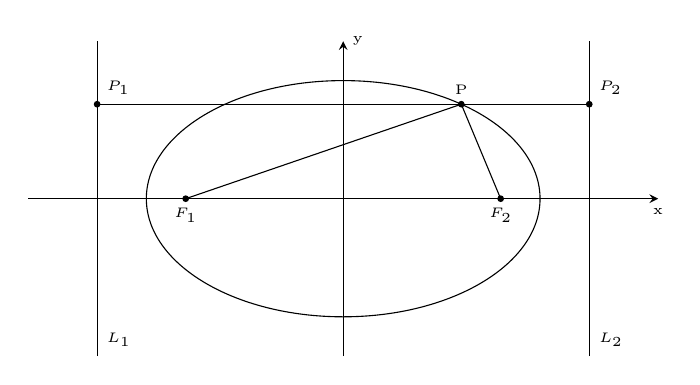
\begin{tikzpicture}
    \draw [->,>=stealth](-4,0)--(4,0) node [anchor=north]{\tiny x};
    \draw [->,>=stealth](0,-2)--(0,2) node [anchor=west]{\tiny y};
    \filldraw (2,0) circle [radius=1pt] node [anchor=north]{\tiny $F_2$};
    \filldraw (-2,0) circle [radius=1pt] node [anchor=north]{\tiny $F_1$};
    \draw(-3.125,-2)--(-3.125,2);
    \draw(3.125,-2)--(3.125,2);
    \draw (0,0) ellipse (2.5 and 1.5);
    \draw (-2,0)--(1.5,1.2)--(2,0);
    \filldraw (1.5,1.2) circle [radius=1pt] node [anchor=south]{\tiny P};
    \draw (-3.125,1.2)--(3.125,1.2);
    \filldraw (-3.125,1.2) circle [radius=1pt] node [anchor=south west] {\tiny $P_1$};
    \filldraw (3.125,1.2) circle [radius=1pt] node [anchor=south west] {\tiny $P_2$};
    \draw (-3.125,-2)node [anchor=south west] {\tiny $L_1$};
    \draw (3.125,-2)node [anchor=south west] {\tiny $L_2$};
  \end{tikzpicture}
  \caption{椭圆}
  \label{fig:tuoyuan}
\end{figure}

\begin{gather}
  \intertext{椭圆的标准解析方程为} 
  \frac{x^2}{a^2}+\frac{y^2}{b^2}=1
  \label{eq:tuoyuan}
  \intertext{准线方程为}
  \left\{
    \begin{gathered}
      l_1:x_1=-\frac{a^2}{c}\\
      l_2:x_2=\frac{a^2}{c}
    \end{gathered}
  \right.
  \intertext{定和性质:}
  |PF_1|+|PF_2|=2a
  \intertext{定比性质:}
  \frac{|PF_1|}{|PP_1|}=\frac{|PF_2|}{|PP_2|}=e=\frac{c}{a}
  \intertext{e为离心率.过椭圆上一点$(x_0,y_0)$的切线方程:}
  \frac{xx_0}{a^2}+\frac{yy_0}{b^2}=1
  \intertext{记斜率为k,则切线的斜率和切点间的关系为}
  k\cdot\frac{y_0}{x_0}=-\frac{b^2}{a^2}
  \intertext{一般高中常用联立方程的形式求$x_1+x_2$,$y_1+y_2$,$x_1x_2$,$y_1y_2$.高考中数学大题必出此类型,从对称的观点可以证明下式成立.}
  \left\{
    \begin{gathered}
      \frac{x^2}{a^2}+\frac{y^2}{b^2}=1\\
      Ax+By+C=0 
    \end{gathered}
  \right.
  \intertext{由直线解得$y=-\frac{Ax+C}{B}$代入椭圆方程可得}
  (A^2a^2+B^2b^2)x^2+Aa^22Cx+a^2(C^2-B^2b^2)=0
  \intertext{注意上式是极其对称的,为了快速解题,需要同学位根据对称的特点背过.其判别式为}
  \Delta_x=4a^2b^2B^2(A^2a^2+B^2b^2-C^2)
  \intertext{于是判定直线与椭圆有无交点只需判断$A^2a^2+B^2b^2$与$C^2$的大小关系即可.}
  A^2a^2+B^2b^2>C^2
  \intertext{上式成立则有两个交点}
  A^2a^2+B^2b^2=C^2
  \intertext{上式成立则有一个交点}
  A^2a^2+B^2b^2<C^2
  \intertext{上式成立则无交点,同时基于x,y的同等地位和对称性,易写出关于y的联立方程式和判别式}
  \left\{
    \begin{gathered}
      (A^2a^2+B^2b^2)y^2+Bb^22Cy+b^2(C^2-A^2a^2)=0\\
      \Delta_y=4a^2b^2A^2(A^2a^2+B^2b^2-C^2)
    \end{gathered}
  \right.
  \intertext{显然由韦达定理易得$x_1+x_2$,$y_1+y_2$,$x_1x_2$,$y_1y-2$之值,此不再赘述.下面再来看一看弦长的问题.一般的x方程为:}
  (x-x_1)(x-x_2)=0\notag\\
  x^2-(x_1+x_2)x+x_1x_2=0\notag\\
  \Delta_x=(x_1+x_2)^2-4x_1x_2=(x_1-x_2)^2
  \intertext{同理}
  \Delta_y=(y_1-y_2)^2
  \intertext{所以有弦长l为}
  l=\sqrt{(x_1-x_2)^2+(y_1-y_2)^2}=\sqrt{\Delta_x+\Delta_y}\notag
  \intertext{代入$\Delta_x$和$\Delta_y$解得}
  l=\frac{2ab}{A^2a^2+B^2b^2}\sqrt{(A^2+B^2)(A^2a^2+B^2b^2-C^2)}
\end{gather}
\subsection{双曲线}
\begin{gather}
  \intertext{双曲线的标准方程为}
  \frac{x^2}{a^2}-\frac{y^2}{b^2}=1
  \intertext{准线方程为}
  \begin{gathered}
    l_1:x_1=-\frac{a^2}{c}\\
    l_2:x_2=\frac{a^2}{c}
  \end{gathered}
  \intertext{定差性质}
  |PF_1|-|PF_2|=2a
  \intertext{定比性质}
  \frac{|PF_1|}{|PP_1|}=\frac{|PF_2|}{|PP_2|}=e=\frac{c}{a}
  \intertext{e为离心率.过双曲线上一点$(x_0,y_0)$的切线方程:}
  \frac{xx_0}{a^2}-\frac{yy_0}{b^2}=1
  \intertext{记斜率为k,则切线的斜率和切点间的关系为}
  k\cdot\frac{y_0}{x_0}=\frac{b^2}{a^2}
  \intertext{将椭圆中$b^2$换成$-b^2$则一切结论适用}
  \left\{
    \begin{gathered}
      \frac{x^2}{a^2}-\frac{y^2}{b^2}=1\\
      Ax+By+C=0 
    \end{gathered}
  \right.
  \intertext{其关于x的联立方程和判别式为}
  \left\{
    \begin{gathered}
      (A^2a^2+B^2b^2)x^2+Bb^22Cx+b^2(C^2-A^2a^2)=0\\
      \Delta_x=-4a^2b^2A^2[(A^2a^2-B^2b^2)-C^2]
    \end{gathered}
  \right.
  \intertext{其根的判断依据为}
  A^2a^2-B^2b^2>C^2
  \intertext{若上式成立则无交点}
  A^2a^2-B^2b^2=C^2
  \intertext{若上式成立则有一个交点}
  A^2a^2-B^2b^2<C^2
  \intertext{若上式成立则有二个交点,其弦长方程为}
l=\frac{2ab}{|A^2a^2-B^2b^2|}\sqrt{(A^2+B^2)[(A^2a^2-B^2b^2)-C^2]}
\end{gather}
\subsection{抛物线}
\begin{gather}
  \intertext{抛物线的标准方程为}
  y^2=2px
  \intertext{准线方程}
  l:x=-\frac{p}{2}
  \intertext{焦点}
  F:x=\frac{p}{2}
  \intertext{切线方程}
  y_0y=2p\cdot\frac{x_0+x}{2}
  \intertext{抛物线和直线方程的联立}
  \begin{gathered}
    y^2=2px\\
    Ax+By+C=0
  \end{gathered}
  \intertext{此方程换成关于y的方程相对简单,即}
  \frac{A}{2p}y^2+By+C=0
  \intertext{根的和与积}
  \begin{gathered}
    y_1+y_2=-\frac{2Bp}{A}\\
    y_1y_2=\frac{2Cp}{A}\\
    x_1+x_2=-\frac{1}{A}[B(y_1+y_2)+2C]\\
    x_1x_2=\frac{4p^2}(y_1y_2)^2
  \end{gathered}
  \intertext{弦长方程为}
  l=\sqrt{(x_1-x_2)^2+(y_1-y_2)^2}\notag\\
  l=\sqrt{1+\left(\frac{x_1-x_2}{y_1-y_2}\right)^2}\sqrt{(y_1-y_2)^2}\notag\\
  l=\sqrt{\left(1+\frac{B^2}{A^2}\right)\left[\left(\frac{2Bp}{A}\right)^2-2\cdot\frac{2Cp}{A}\right]}
  \intertext{抛物线的规律比较简单,但是公式的结果不如椭圆和双曲线对称,认真分析以上结果的对称性,针对这一部分的习题应该能较快的做出结果来.}
\end{gather}
\subsection{一般圆锥曲线方程的切线方程}
\begin{gather}
  \intertext{ 一般的圆锥曲线方程的切线方程为}
  Ax^2+By^2+Cxy+Dx+Ey+F=0
  \intertext{曲线上任意一点$(x_0,y_0)$,则过此点的切线方程为}
  Ax_0x+By_0y+C\frac{x_0y+xy_0}{2}+D\frac{x+x_0}{2}+E\frac{y+y_0}{2}+F=0
  \intertext{例如曲线$xy=1$其上一点$(x_0,y_0)$处切线为}
  \frac{x_0y+xy_0}{2}=1
  \intertext{对于一般圆锥曲线方程,利用转轴公式可以化到标准曲线方程,高中不再讨论转轴公式,此处略去.仅指明计算方法.另外一点要提醒的是,讨论离心率一定要用下面的形式计算,则可以简化计算}
  \begin{gathered}
    \mbox{椭圆:} e=\sqrt{1-\frac{b^2}{a^2}}\\
    \mbox{双曲线:} e=\sqrt{1+\frac{b^2}{a^2}}
  \end{gathered}
  \intertext{简化计算的原因在于因子$\frac{b^2}{a^2}$可以约去公因子.}\notag
\end{gather}
\subsection{圆锥曲线的参数解法}

\begin{gather}
  \intertext{椭圆和直线联立的方程为}
  \begin{gathered}
    \frac{x^2}{a^2}+\frac{y^2}{b^2}=1\\
    Ax+By+C=0
  \end{gathered}
  \intertext{取椭圆的参数方程}
  \begin{gathered}
    x=a\cos\theta\\
    y=b\sin\theta
  \end{gathered}
  \intertext{将上式代入直线方程,则}
  Aa\cos\theta+Bb\sin\theta+C=0
  \intertext{取辅助角为}
  \begin{gathered}
    \sin\alpha=\frac{Aa}{\sqrt{A^2a^2+B^2b^2}}\\
    \cos\alpha=\frac{Bb}{\sqrt{A^2a^2+B^2b^2}}
  \end{gathered}
  \intertext{所以得}
  \sqrt{A^2a^2+B^2b^2}\cdot\sin(\theta+\alpha)+C=0
  \intertext{由上式求得}
  \sin(\theta+\alpha)=-\frac{C}{\sqrt{A^2a^2+B^2b^2}}
  \intertext{如果上式成立,则直线与方程有交点.进而得到有交点的条件为}
  A^2a^2+B^2b^2\geqslant C^2
  \intertext{在有交点的前提下,可以求得}
  \begin{gathered}
    \cos\theta=\cos(\theta+\alpha-\alpha)=\cos(\theta+\alpha)\cos\alpha+\sin(\theta+\alpha)\sin\alpha\\
    \cos\theta=-\frac{1}{A^2a^2+B^2b^2}(AaC\pm Bb\sqrt{(A^2a^2+B^2b^2)-C^2})\\
    \sin\theta=\sin(\theta+\alpha-\alpha)=\sin(\theta+\alpha)\cos\alpha+\cos(\theta+\alpha)\sin\alpha\\
    \sin\theta=-\frac{1}{A^2a^2+B^2b^2}(BbC\pm Aa\sqrt{(A^2a^2+B^2b^2)-C^2})
  \end{gathered}
  \intertext{将$\cos\theta$和$\sin\theta$代入参数方程,得交点为}
  \begin{gathered}
  x=-\frac{a}{A^2a^2+B^2b^2}(AaC\pm Bb\sqrt{(A^2a^2+B^2b^2)-C^2})\\
  y=-\frac{b}{A^2a^2+B^2b^2}(BbC\pm Aa\sqrt{(A^2a^2+B^2b^2)-C^2})
  \end{gathered}
  \intertext{于是立刻得二个交点的和与积}
  \begin{gathered}
    x_1+x_2=-\frac{2Aa^2C}{A^2a^2+B^2b^2}\\
    x_1x_2=\frac{a^2(C^2-B^2b^2)}{A^2a^2+B^2b^2}
  \end{gathered}
  \intertext{所以得关于x的联立方程}
  (A^2a^2+B^2b^2)x^2+Aa^22Cx+a^2(C^2-B^2b^2)=0
  \intertext{基于x和y的对称性可得}
  (A^2a^2+B^2b^2)y^2+Bb^22Cy+b^2(C^2-A^2a^2)=0
  \intertext{对于双曲线,则只需在椭圆的基础上将$b$代换成$ib$便得到双曲线方程}
  \begin{gathered}
    \frac{x^2}{a^2}+\frac{y^2}{(ib)^2}=1\\
    \frac{x^2}{a^2}-\frac{y^2}{b^2}=1
  \end{gathered}
  \intertext{它和直线的联立方程为}
  \begin{gathered}
  (A^2a^2-B^2b^2)x^2+Aa^22Cx+a^2(C^2+B^2b^2)=0\\
  (A^2a^2-B^2b^2)y^2-Bb^22Cy-b^2(C^2-A^2a^2)=0
  \end{gathered}
  \intertext{双曲线与直线的交点为}
  \begin{gathered}
    x=-\frac{a}{A^2a^2-B^2b^2}(AaC\pm Bib\sqrt{(A^2a^2-B^2b^2)-C^2})\\
    y=-\frac{ib}{A^2a^2-B^2b^2}(BibC\pm Aa\sqrt{(A^2a^2-B^2b^2)-C^2})
  \end{gathered}
  \intertext{显然,若要根为实根,则根号内必为负值才可以消去虚数单位,}
  \begin{gathered}
    x=-\frac{a}{A^2a^2-B^2b^2}(AaC\mp Bb\sqrt{C^2-(A^2a^2-B^2b^2)})\\
    y=\frac{b}{A^2a^2-B^2b^2}(BbC\pm Aa\sqrt{C^2-(A^2a^2-B^2b^2)})
  \end{gathered}
  \intertext{所以双曲线存在实根的条件为}
   A^2a^2-B^2b^2\leqslant C^2
   \intertext{得到联立方程后,则其它一切问题就好解决了,此处不再赘述.}\notag
\end{gather}
